\subsection{Optimization for the low density
scenario}\label{subsec:ldoptimization}

Also in this case, we have run a full factorial analysis, with low values of
each parameter, in order to identify the minimum values required to reach the
coverage. Each possible configuration (\(750\)) has been run with 10
repetitions. The complete analysis can be found in \code{coverage.ipynb}. The
configuration used is named ``LowDensityCoverage''. We have found out that to
reach at least the \(99\%\) of the coverage, we need to have a broadcast radius
of at least \(23m\), but we also need higher values for \(m\) and \(D\). If we
use \(R\!=\!25m\) we get better results for the other parameters. In particular,
we have found the following minimum configuration the we consider ``good'' and
``well balanced'' since it does not use the value \code{1} for any of the
parameters.

\begin{center}
	\begin{tabular}{cccc}
		\toprule
		R & T & m & \(\max(\delta)\) \\
		\midrule
		\(25m\) & \(2s\) & \(2\,\mathit{copies}\) & \(2s\) \\
		\bottomrule
	\end{tabular}
\end{center}

As in the high density scenario, to optimize the \standout{total broadcast time}
we need to increase the broadcast radius or decrease the size of the hear
window. The results are in the file \code{broadcast-time.ipynb}. The
configuration used is named ``LowDensityTime'', where we use, as suggested from
the plots of \code{2kr.ipynb}, high values for \(m\) and low value for the
maximum relay delay. As shown in \figref{fig:ldtimeff}, we see that with low
values of T we can reduce a lot the broadcast time (as expected). If we do not
want to sacrifice the energy efficiency, it is convenient to only reduce the
hear window, without increasing the radius (also increase a just a little \(R\)
is not convenient because there isn't a big difference in the time).

\begin{figure}[hbt]
	\centering
	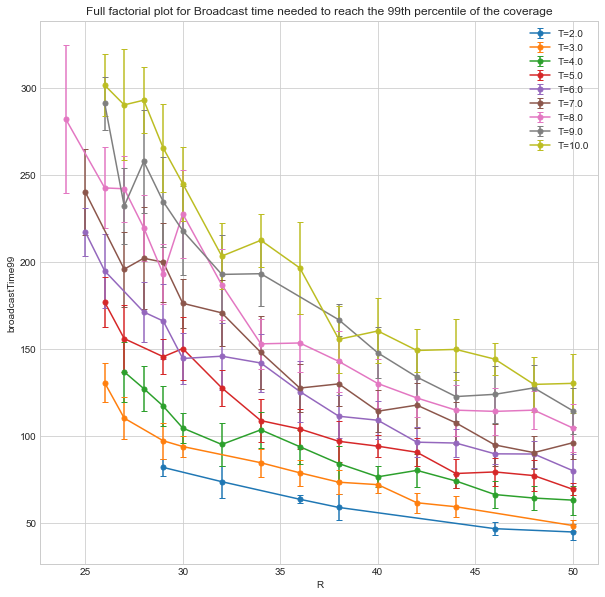
\includegraphics[width=0.6\textwidth]{img/ld/broadcasttime-R-ffplot}
	\caption{The broadcast time is lower with higher values of the broadcast
	radius and lower values of the size of the hear
	window (95\% confidence intervals)}\label{fig:ldtimeff}
\end{figure}

To optimize the \standout{energy efficiency}, we have to study the number of
messages. The analysis can be found in \code{messages.ipynb}. We use low values
for the broadcast radius (that obviously improves energy efficiency). Other
factors taken into considerations are the one we have identified as relevant in
\secref{subsec:ld2kr}, namely the maximum number of copies and the size of the
hear window. The configuration used is named ``LowDensityMessages''.

As we can see from \figref{fig:ldmessagesff}, we get that the maximum number of
copies hugely affects the total number of messages sent, as previously found by
the \(2^{k}r\) analysis. Also increasing the size of the hear window have
benefits (but lower benefits, as found by the \(2^{k}r\)).

\begin{figure}[htb]
	\centering
	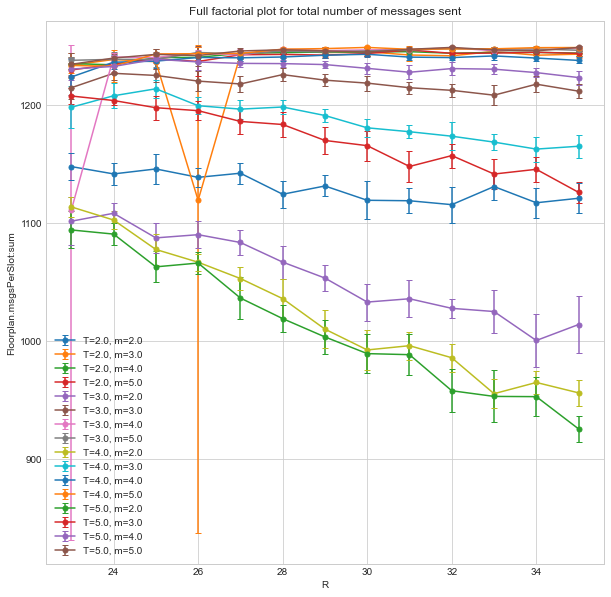
\includegraphics[width=0.7\textwidth]{img/ld/messages-R-ffplot.png}
	\caption{With low values of the maximum number of copies and higher
	values for the size of the hear window, we get a lower number of
	messages sent}\label{fig:ldmessagesff}
\end{figure}

So, in order to improve the energy efficiency, since we can not increase the
broadcast radius, we need to use surely low values for \(m\) and also an higher
\(T\). Increasing \(T\) also increases the broadcast time, so a trade-off
decision is needed in this parameter. Because manipulating the hear window we
have only little benefits in the energy consumption, we can decide to use a low
or medium value, which implies a little bit more of consumption but a large
benefit in the broadcast time.

Regarding the \standout{total number of collisions}, we can reduce it by
reducing the broadcast radius and the maximum number of copies. Also helps
increasing the maximum relay delay, such as in the high density scenario.
Factorial analysis with the \(m\) and \(\max(\delta)\) parameters is available
in \code{collisions.ipynb}, using the configuration named
``LowDensityCollisions''. \figref{fig:ldcollisionsff} shows the results:
increasing \(\max(\delta)\) should allow to have even a lower number of
collisions. \(m\!=\!2\) is a good setup for this parameter since it allows to
completely exploit the advantages of the \emph{trickle relaying} algorithm in
order to reduce the number of collisions and the number of messages sent.

\begin{figure}[htb]
	\centering
	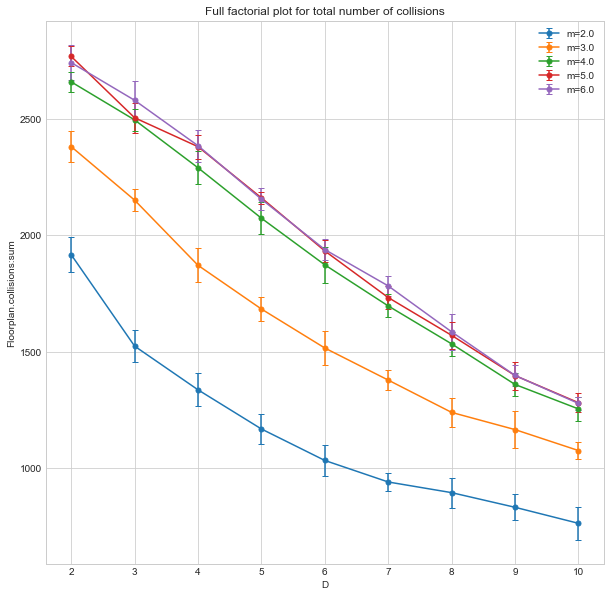
\includegraphics[width=0.5\textwidth]{img/ld/collisions-D-ffplot}
	\caption{The number of collisions is linearly dependent on the maximum
	relay delay. Also, trickle relaying can be exploited with low values of
	\(m\) in order to reduce the number of
	collisions}\label{fig:ldcollisionsff}
\end{figure}

\subsubsection{Conclusions}\label{subsubsec:ldconclusions}

\begin{itemize}
	\item The minimal configuration to get a nearly perfect coverage is with
		\(R\!=\!25m\), \(T\!=\!2s\), \(m\!=\!2\) and
		\(\max(\delta)\!=\!2s\). Higher values for these parameters does
		not break the coverage.
	\item If a low total broadcast time is a main objective, increasing
		\(R\) is effective, but is better to reduce \(T\).
	\item If instead a better energy efficiency is the main objective, \(R\)
		can not be increased and \(T\) should not be reduced. A
		trade-off decision between a low broadcast time and a good
		energy efficiency is needed. We have to consider that for this
		configuration changing \(T\) has a greater influence for the
		broadcast time than the one related to the number of messages.
	\item Also in this configuration \(m\!=\!2\) is perfect to have a lower
		number of collisions and a better energy efficiency without
		sacrificing the broadcast time, thanks to trickle relaying.
	\item \(\max(\delta)\) should be high, in order to reduce the total
		number of collisions, but not too much, in order to avoid an
		increase in the broadcast time due to users waiting time.
\end{itemize}
